\section{The Heisenberg model}


\begin{figure}[H]
  \begin{center}
    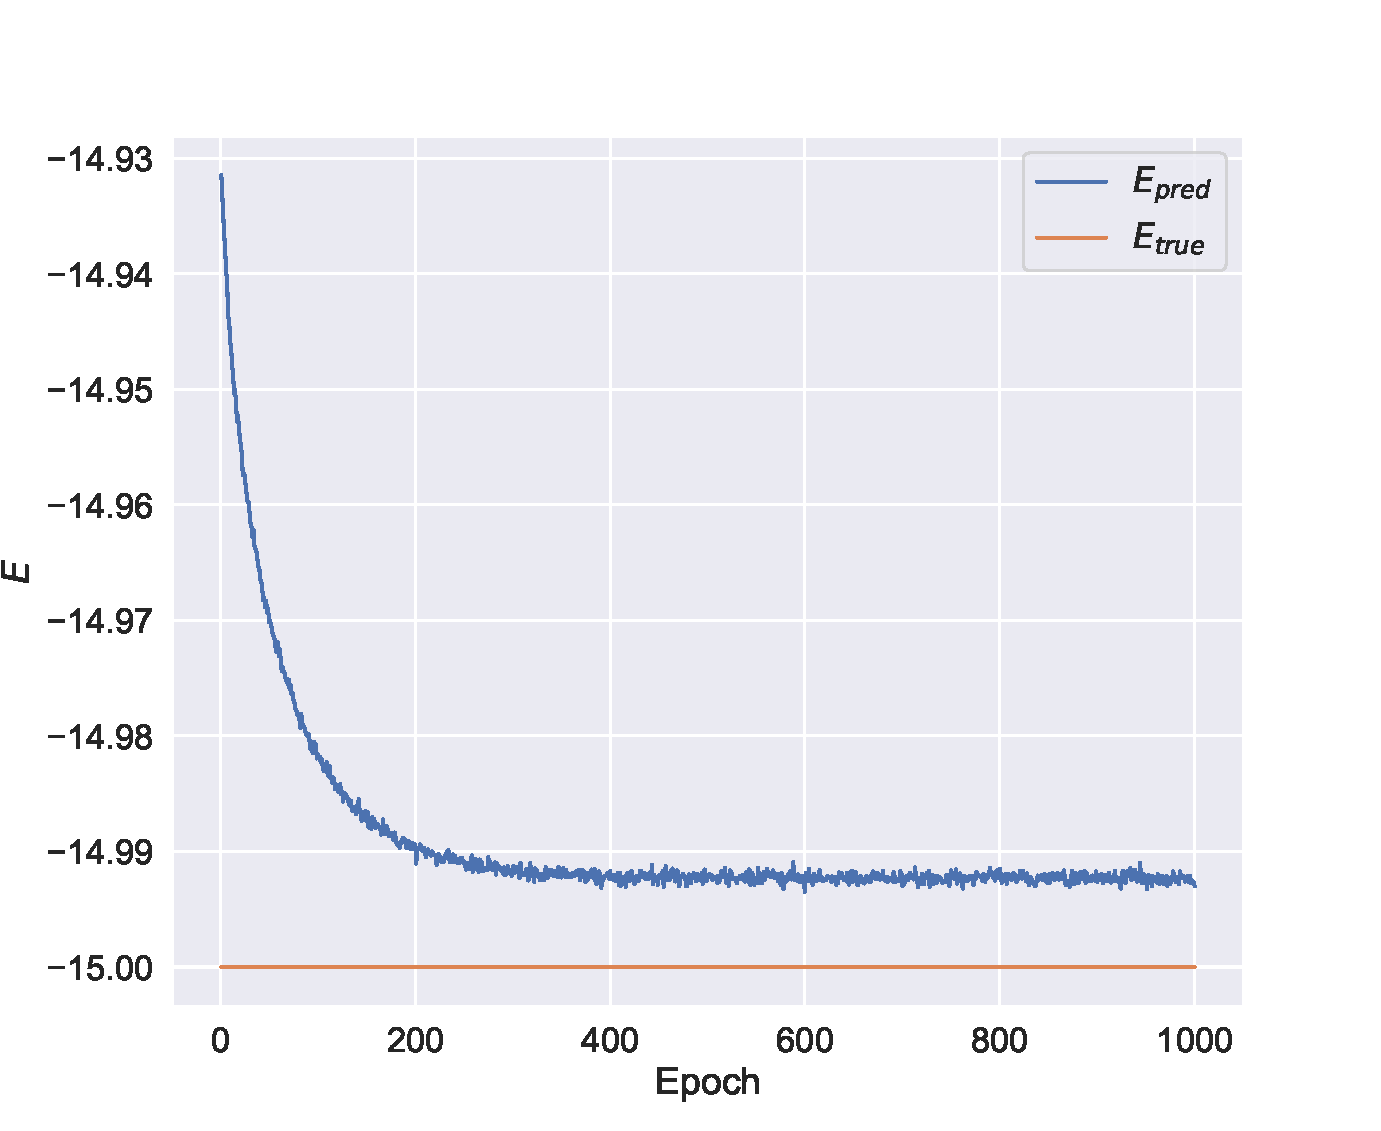
\includegraphics[width=0.95\textwidth]{Figures/Plots/Heisen/heisen_conv10}
  \end{center}
  \caption{The convergence graph of the RBM mean energy output for the Heisenberg model with $N = 10$ particles, $M=1$, and $J=-1$ and $L=-0.5$.}
\end{figure}

And the two-dimensional Heisenberg model results in the following convergence graph:

\begin{figure}[H]
  \begin{center}
    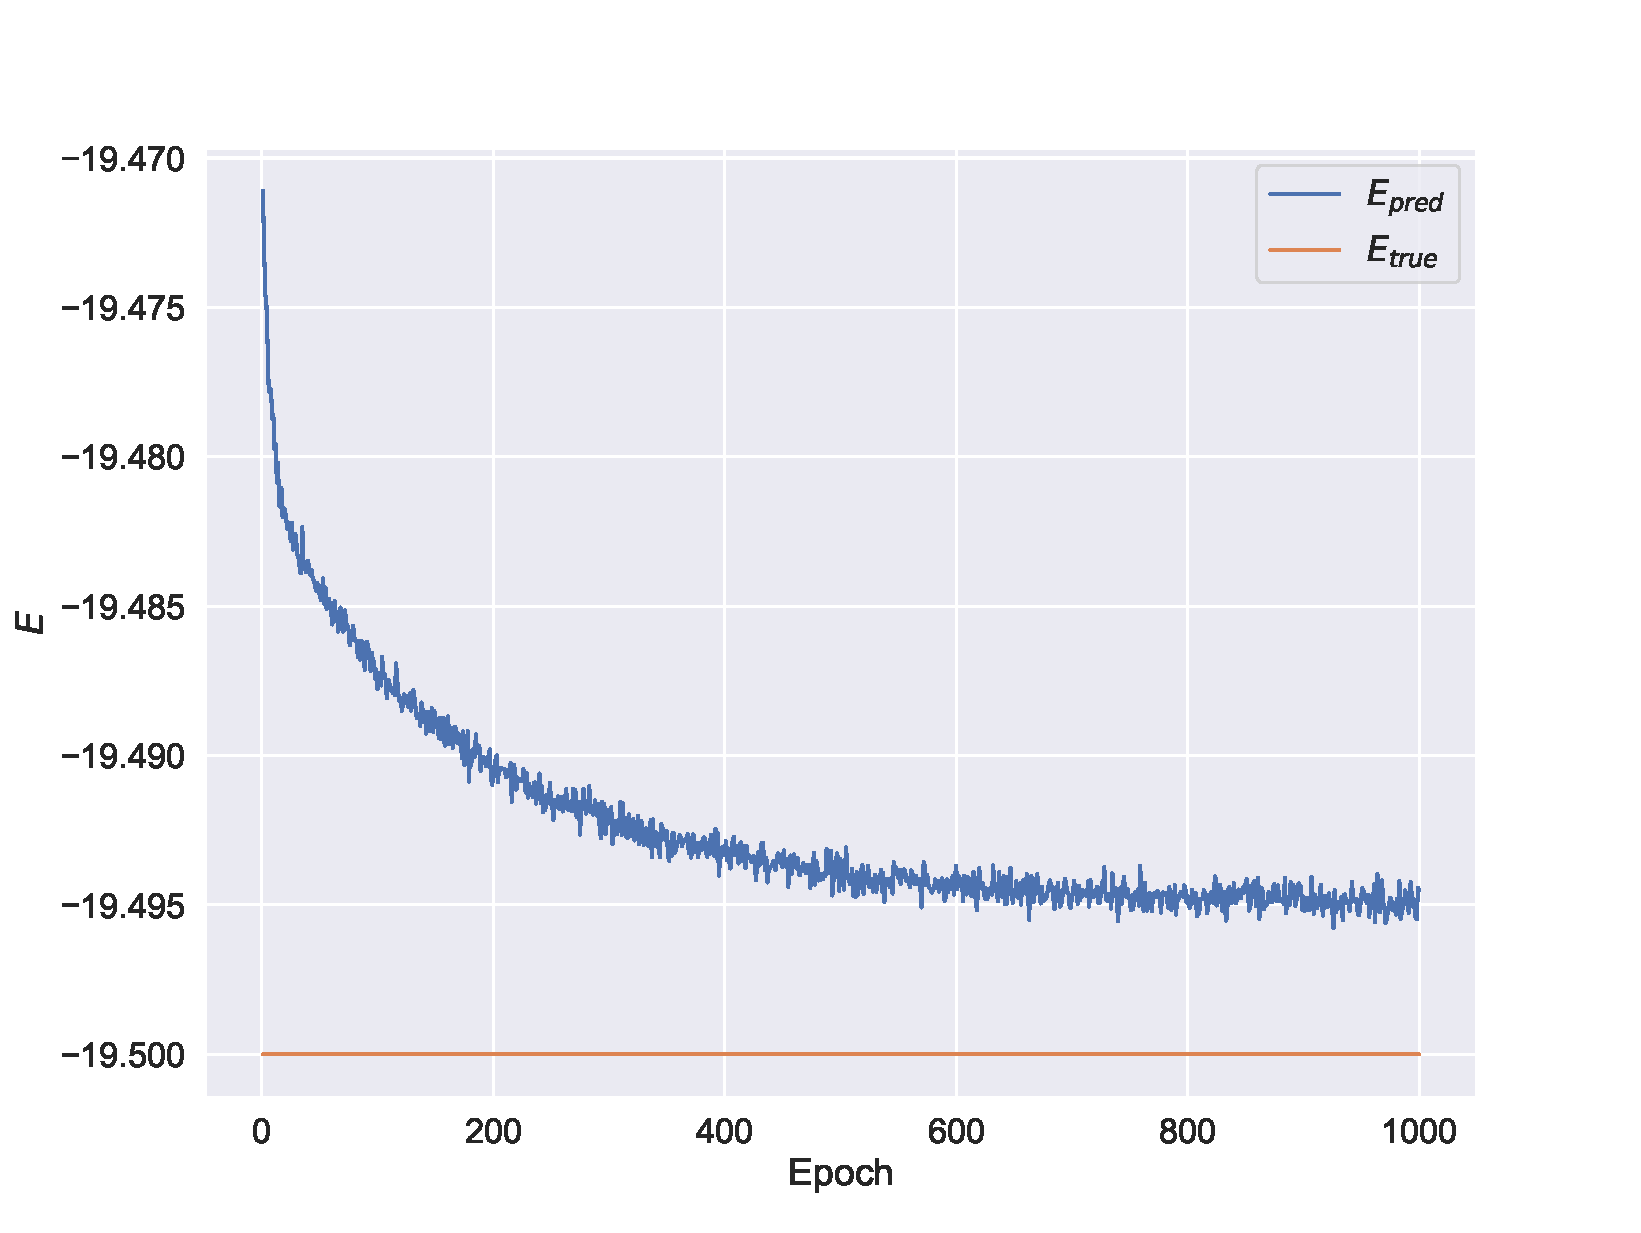
\includegraphics[width=0.95\textwidth]{Figures/Plots/Heisen/heisen_conv33}
  \end{center}
  \caption{The convergence graph of the RBM mean energy output for the two-dimensional Heisenberg model with $N = 3$ particles, $M=3$, and $J=-1$ and $L=-0.5$.}
\end{figure}

For both of these, but espacially the two-dimensional case, the initialized machine state has a energy close to the ground state energy, and the convergence graph there appears more unstable than the ones for the lipkin and Ising model previously. For the Heisenberg model the number of epochs has been increased to a thousand, as for the two-dimensional case we see a clear increase in convergence time.

\subsection{The effect of \texorpdfstring{$J$}{J} on RBM prediction accuracy}

For one dimension with $10$ lattice points and $L=-0.5$ we get the following:

\begin{figure}[H]
  \begin{center}
    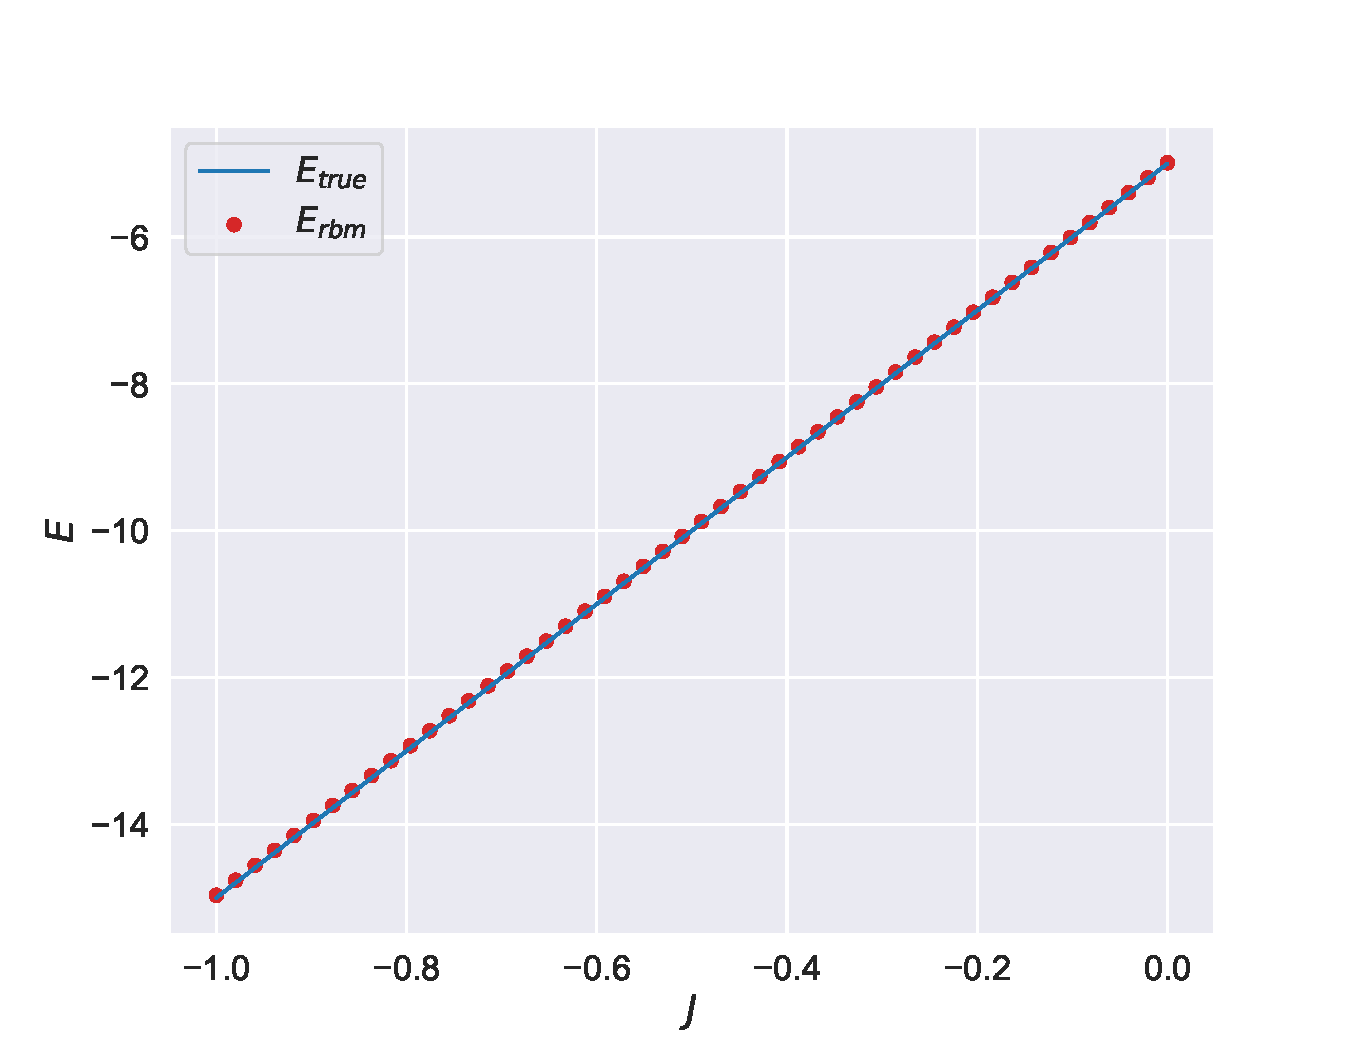
\includegraphics[width=0.95\textwidth]{Figures/Plots/Heisen/val-true[J][-1.0-0.0][e=500][n=10][N=10][M=1][L=-0.5]}
  \end{center}
  \caption{The true ground state energy together with the restricted Boltzmann machine local energy output for the Heisenberg model with $10$ lattice points and $L=-0.5$.}
\end{figure}

And looking at the two-dimensional version we get

\begin{figure}[H]
  \begin{center}
    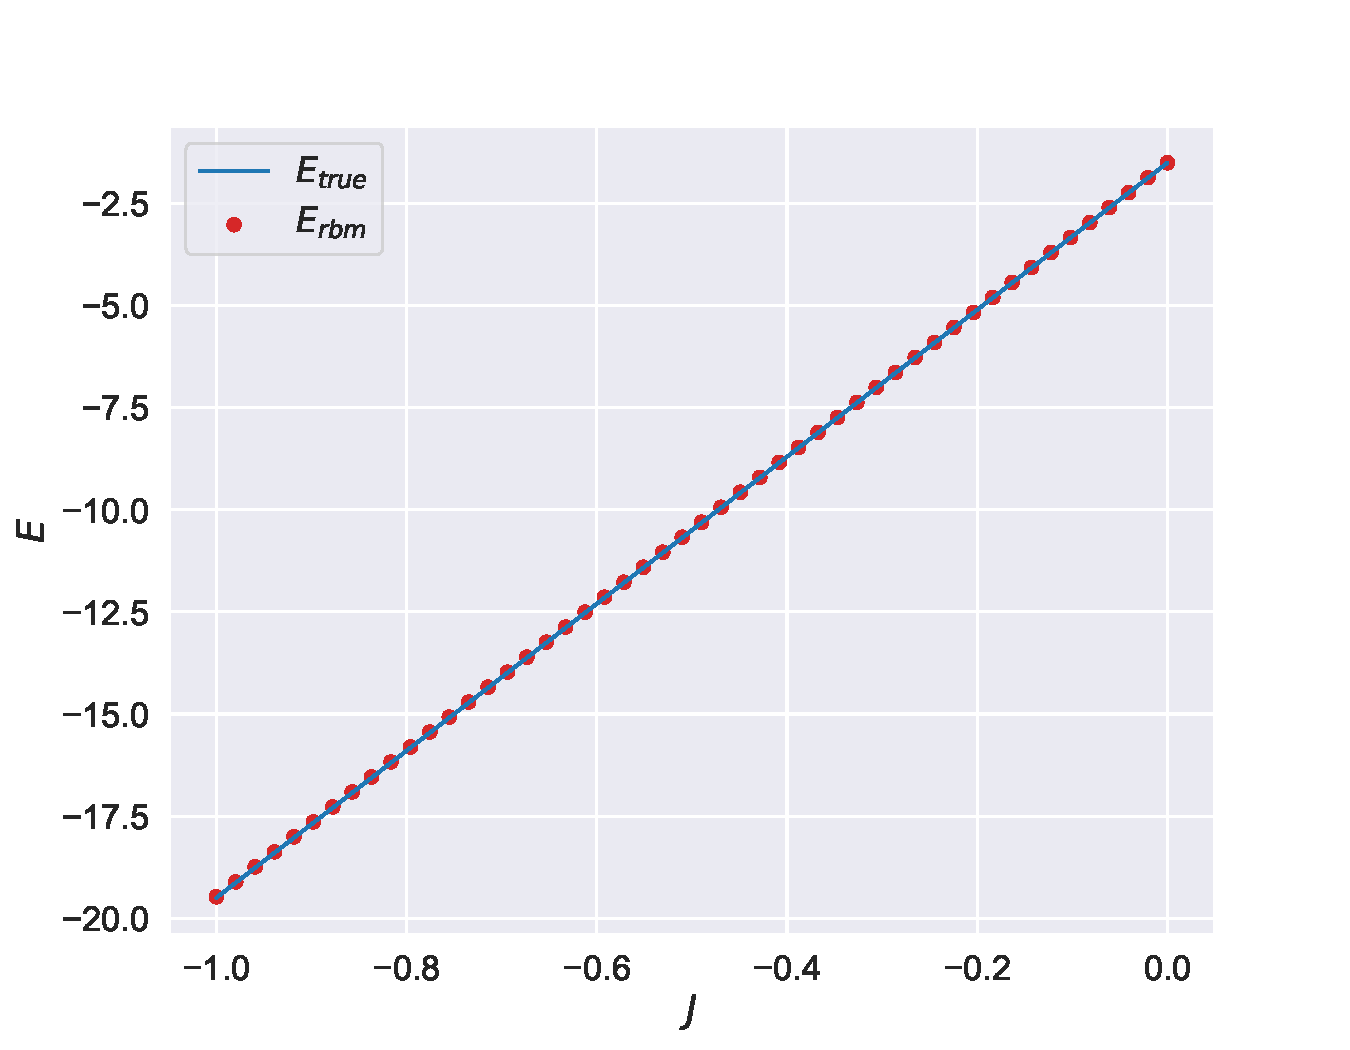
\includegraphics[width=0.95\textwidth]{Figures/Plots/Heisen/val-true[J][-1.0-0.0][e=500][n=9][N=3][M=3][L=-0.5]}
  \end{center}
  \caption{The true ground state energy together with the restricted Boltzmann machine local energy output for the two-dimensional Heisenberg model with $9$ lattice points, $N=3$ and $M=3$, and $L=-0.5$.}
\end{figure}

For both the one-dimensional and two-dimensional case the RBM manages to predict the ground state energy well without any of the behaviour seen witht he Ising model.

\subsection{The effect of \texorpdfstring{$L$}{L} on RBM prediction accuracy}

\begin{figure}[H]
  \begin{center}
    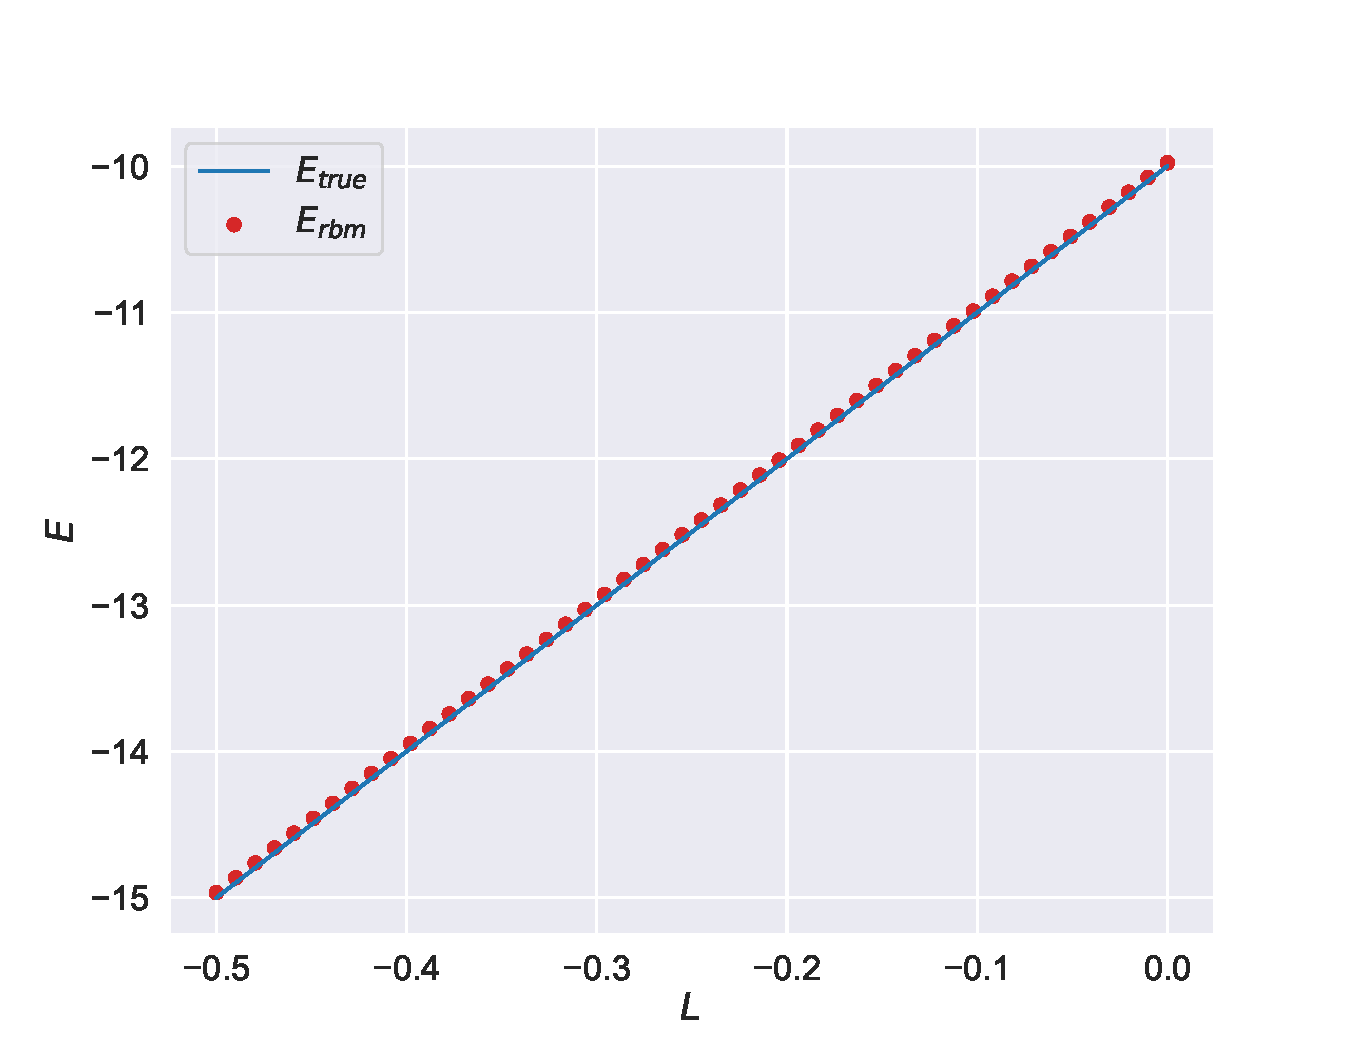
\includegraphics[width=0.95\textwidth]{Figures/Plots/Heisen/val-true[L][-0.5-0.0][e=500][n=10][N=10][M=1][J=-1]}
  \end{center}
  \caption{The true ground state energy together with the restricted Boltzmann machine local energy output for the Heisenberg model with $10$ lattice points and $J=-1$.}
\end{figure}

And with two dimensions

\begin{figure}[H]
  \begin{center}
    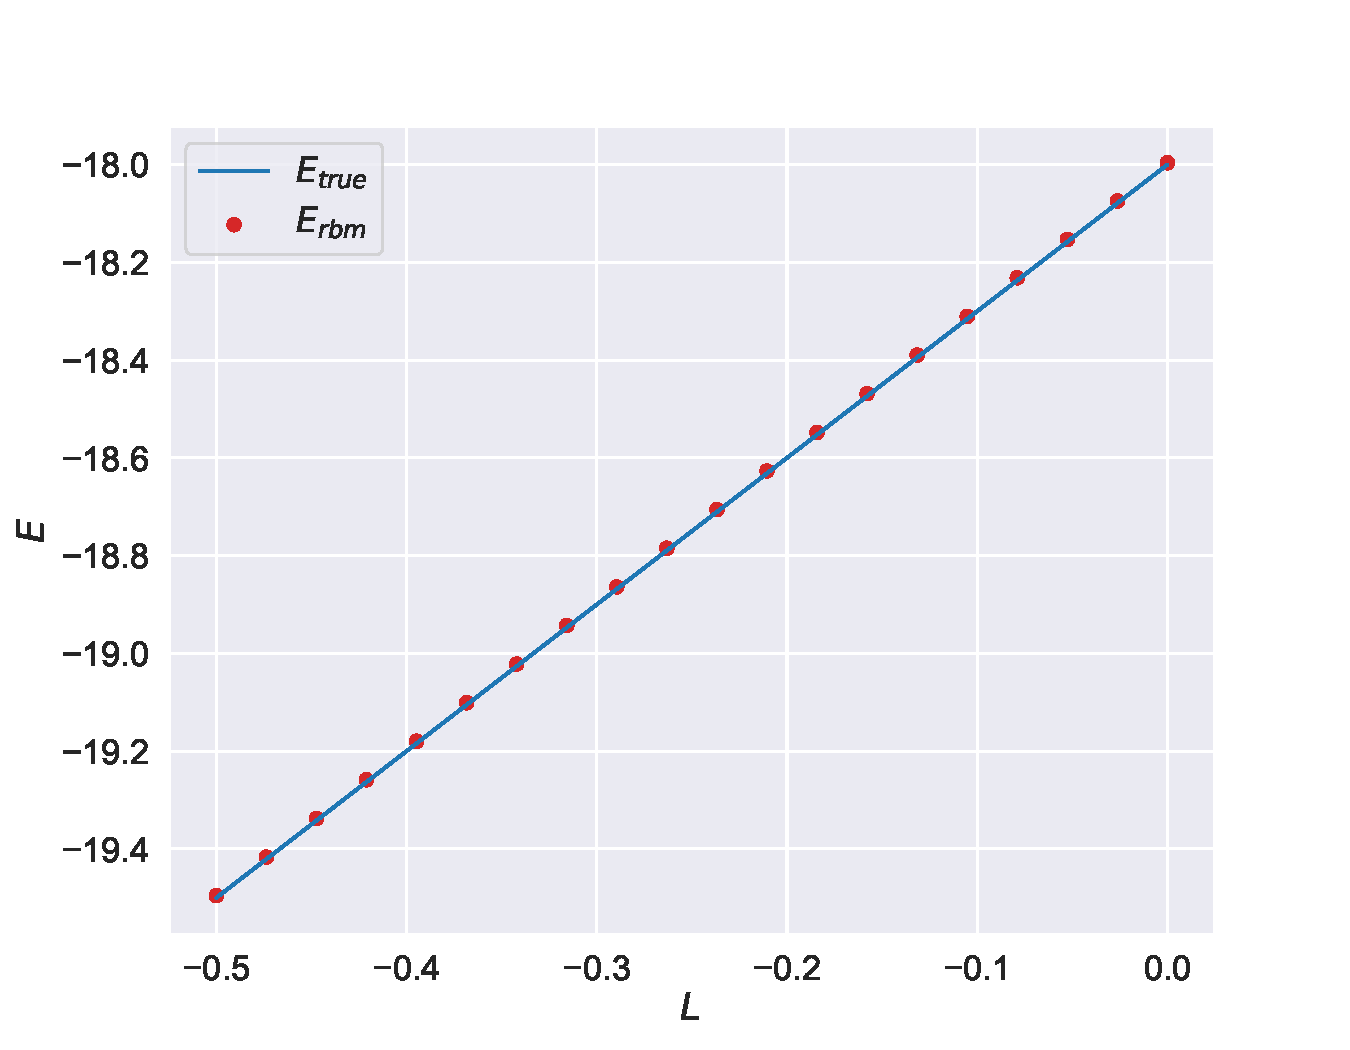
\includegraphics[width=0.95\textwidth]{Figures/Plots/Heisen/val-true[L][-0.5-0.0][e=1000][n=9][N=3][M=3][J=-1]}
  \end{center}
  \caption{The true ground state energy together with the restricted Boltzmann machine local energy output for the Heisenberg model with $9$ lattice points, $N=3$ and $M=3$, and $J=-1$.} 
\end{figure}

For the one-dimensional case we see the RBM prediction being slightly above the true ground state energy, though for both we see a consistent accuracy for the whole range.

